\section{Results}
\label{sec:-res}
We find that our model of user accuracy is accurate within bounds
%\begin{figure}
%  \input{plots/relations}
%  \caption{}\label{fig:-rel}
%\end{figure}

\begin{figure}[bht]
\centering
 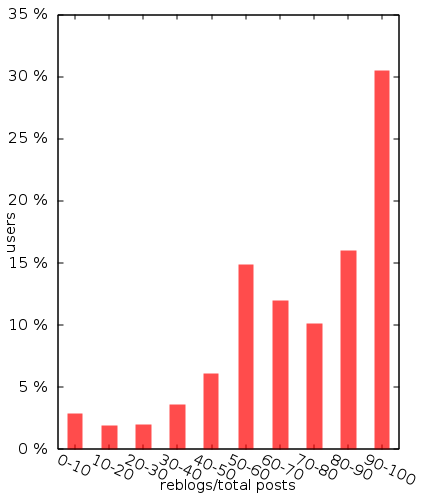
\includegraphics[width=3.5in]{degree}
  \caption{The bins on the X axis represent percentages of users, grouped by what percentage of their posts are reblogs.  The Y axis indicates the magnitude of the membership within this group.  Overall, we observe that blogs contain an average of 70\% reblogged material, and a median amount of 76\% reblogged material.}
  \label{fig:-deg}
\end{figure}

This figure indicates that there are very few users that contribute 
primarily original content.  These results indicate 

We find that approximately 15\% of all users generate more original 
content than they repost.  By contrast, 15\% of users post around half 
original content, 30\% repost almost exclusively, and another 40\% or 
so does a considerably higher amount of reblogging than original 
blogging.

We find that the most popular type of post on Tumblr is the
gifsets\cite{hillman2014tumblr}

\begin{figure}[bht]
\centering
 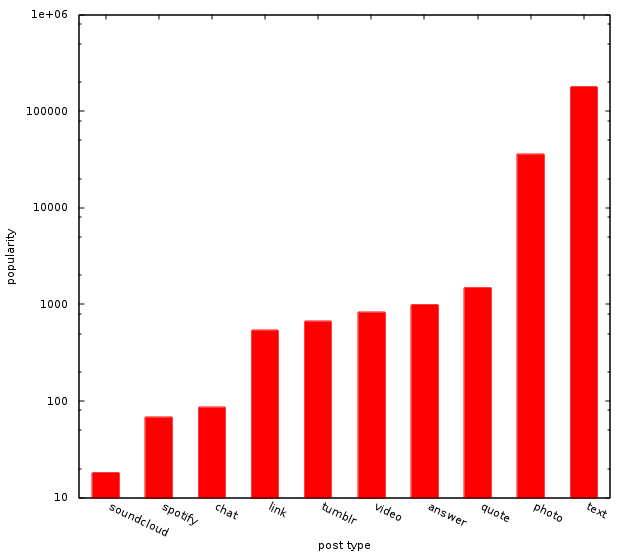
\includegraphics[width=3.5in]{popularity}
  \caption{The graph represents the relative popularity of all surveyed post types.  Note that the graph has a log scale on the y axis}
  \label{fig:-pop}
\end{figure}
This is particularly interesting in light of the 

%%% Local Variables: 
%%% mode: latex
%%% TeX-master: "main"
%%% End: 
